
%% bare_jrnl.tex
%% V1.4b
%% 2015/08/26
%% by Michael Shell
%% see http://www.michaelshell.org/
%% for current contact information.
%%
%% This is a skeleton file demonstrating the use of IEEEtran.cls
%% (requires IEEEtran.cls version 1.8b or later) with an IEEE
%% journal paper.
%%
%% Support sites: %% http://www.michaelshell.org/tex/ieeetran/
%% http://www.ctan.org/pkg/ieeetran
%% and
%% http://www.ieee.org/

%%*************************************************************************
%% Legal Notice:
%% This code is offered as-is without any warranty either expressed or
%% implied; without even the implied warranty of MERCHANTABILITY or
%% FITNESS FOR A PARTICULAR PURPOSE!
%% User assumes all risk.
%% In no event shall the IEEE or any contributor to this code be liable for
%% any damages or losses, including, but not limited to, incidental,
%% consequential, or any other damages, resulting from the use or misuse
%% of any information contained here.
%%
%% All comments are the opinions of their respective authors and are not
%% necessarily endorsed by the IEEE.
%%
%% This work is distributed under the LaTeX Project Public License (LPPL)
%% ( http://www.latex-project.org/ ) version 1.3, and may be freely used,
%% distributed and modified. A copy of the LPPL, version 1.3, is included
%% in the base LaTeX documentation of all distributions of LaTeX released
%% 2003/12/01 or later.
%% Retain all contribution notices and credits.
%% ** Modified files should be clearly indicated as such, including  **
%% ** renaming them and changing author support contact information. **
%%*************************************************************************


% *** Authors should verify (and, if needed, correct) their LaTeX system  ***
% *** with the testflow diagnostic prior to trusting their LaTeX platform ***
% *** with production work. The IEEE's font choices and paper sizes can   ***
% *** trigger bugs that do not appear when using other class files.       ***                          ***
% The testflow support page is at:
% http://www.michaelshell.org/tex/testflow/



\documentclass[journal]{IEEEtran}
%
% If IEEEtran.cls has not been installed into the LaTeX system files,
% manually specify the path to it like:
% \documentclass[journal]{../sty/IEEEtran}





% Some very useful LaTeX packages include:
% (uncomment the ones you want to load)


% *** MISC UTILITY PACKAGES ***
%
%\usepackage{ifpdf}
% Heiko Oberdiek's ifpdf.sty is very useful if you need conditional
% compilation based on whether the output is pdf or dvi.
% usage:
% \ifpdf
%   % pdf code
% \else
%   % dvi code
% \fi
% The latest version of ifpdf.sty can be obtained from:
% http://www.ctan.org/pkg/ifpdf
% Also, note that IEEEtran.cls V1.7 and later provides a builtin
% \ifCLASSINFOpdf conditional that works the same way.
% When switching from latex to pdflatex and vice-versa, the compiler may
% have to be run twice to clear warning/error messages.






% *** CITATION PACKAGES ***
%
%\usepackage{cite}
% cite.sty was written by Donald Arseneau
% V1.6 and later of IEEEtran pre-defines the format of the cite.sty package
% \cite{} output to follow that of the IEEE. Loading the cite package will
% result in citation numbers being automatically sorted and properly
% "compressed/ranged". e.g., [1], [9], [2], [7], [5], [6] without using
% cite.sty will become [1], [2], [5]--[7], [9] using cite.sty. cite.sty's
% \cite will automatically add leading space, if needed. Use cite.sty's
% noadjust option (cite.sty V3.8 and later) if you want to turn this off
% such as if a citation ever needs to be enclosed in parenthesis.
% cite.sty is already installed on most LaTeX systems. Be sure and use
% version 5.0 (2009-03-20) and later if using hyperref.sty.
% The latest version can be obtained at:
% http://www.ctan.org/pkg/cite
% The documentation is contained in the cite.sty file itself.






% *** GRAPHICS RELATED PACKAGES ***
%
\ifCLASSINFOpdf
  % \usepackage[pdftex]{graphicx}
  % declare the path(s) where your graphic files are
  % \graphicspath{{../pdf/}{../jpeg/}}
  % and their extensions so you won't have to specify these with
  % every instance of \includegraphics
  % \DeclareGraphicsExtensions{.pdf,.jpeg,.png}
\else
  % or other class option (dvipsone, dvipdf, if not using dvips). graphicx
  % will default to the driver specified in the system graphics.cfg if no
  % driver is specified.
  % \usepackage[dvips]{graphicx}
  % declare the path(s) where your graphic files are
  % \graphicspath{{../eps/}}
  % and their extensions so you won't have to specify these with
  % every instance of \includegraphics
  % \DeclareGraphicsExtensions{.eps}
\fi
% graphicx was written by David Carlisle and Sebastian Rahtz. It is
% required if you want graphics, photos, etc. graphicx.sty is already
% installed on most LaTeX systems. The latest version and documentation
% can be obtained at:
% http://www.ctan.org/pkg/graphicx
% Another good source of documentation is "Using Imported Graphics in
% LaTeX2e" by Keith Reckdahl which can be found at:
% http://www.ctan.org/pkg/epslatex
%
% latex, and pdflatex in dvi mode, support graphics in encapsulated
% postscript (.eps) format. pdflatex in pdf mode supports graphics
% in .pdf, .jpeg, .png and .mps (metapost) formats. Users should ensure
% that all non-photo figures use a vector format (.eps, .pdf, .mps) and
% not a bitmapped formats (.jpeg, .png). The IEEE frowns on bitmapped formats
% which can result in "jaggedy"/blurry rendering of lines and letters as
% well as large increases in file sizes.
%
% You can find documentation about the pdfTeX application at:
% http://www.tug.org/applications/pdftex


\usepackage{color}
\usepackage{amsmath}
\usepackage{amssymb}
\usepackage{tabularx}

\usepackage{epsfig}
%\usepackage[colorlinks=false, urlcolor=black, pdfborder={0 0 0}]{hyperref}
%\let\url\nolinkurl
%\usepackage[options]{nohyperref}  % This makes hyperref commands do nothing without errors
\usepackage{url}  % This makes \url work

%\usepackage[dvips]{epsfig}
\usepackage{etoolbox}
\apptocmd{\sloppy}{\hbadness 10000\relax}{}{}

\usepackage{longtable}
\usepackage{graphicx}
\usepackage[T1]{fontenc}
\usepackage{paralist}
\usepackage{enumitem}
%%%%%%%%%%%%for
\usepackage{adjustbox}
\usepackage{array}
\usepackage{booktabs}
\newcolumntype{C}{>{\centering\arraybackslash}X} % centered version of "X" type
\setlength{\extrarowheight}{1pt}
\usepackage{lipsum}
\usepackage{multirow}

\newcolumntype{R}[2]{%
    >{\adjustbox{angle=#1,lap=\width-(#2)}\bgroup}%
    l%
    <{\egroup}%
}
\newcommand*\rot{\multicolumn{1}{R{90}{1em}}}% no optional argument here, please!

\usepackage{epstopdf}


\def\BibTeX{{\rm B\kern-.05em{\sc i\kern-.025em b}\kern-.08em
    T\kern-.1667em\lower.7ex\hbox{E}\kern-.125emX}}

\usepackage{pdflscape}
%\usepackage{subfigure}
\usepackage{tabularx}
\usepackage{xtab}
%\usepackage{supertabular}

\usepackage{booktabs, threeparttable}
\usepackage{array}
\newcolumntype{L}[1]{>{\raggedright\arraybackslash}p{#1}}

% *** MATH PACKAGES ***
%
%\usepackage{amsmath}
% A popular package from the American Mathematical Society that provides
% many useful and powerful commands for dealing with mathematics.
%
% Note that the amsmath package sets \interdisplaylinepenalty to 10000
% thus preventing page breaks from occurring within multiline equations. Use:
%\interdisplaylinepenalty=2500
% after loading amsmath to restore such page breaks as IEEEtran.cls normally
% does. amsmath.sty is already installed on most LaTeX systems. The latest
% version and documentation can be obtained at:
% http://www.ctan.org/pkg/amsmath





% *** SPECIALIZED LIST PACKAGES ***
%
%\usepackage{algorithmic}
% algorithmic.sty was written by Peter Williams and Rogerio Brito.
% This package provides an algorithmic environment fo describing algorithms.
% You can use the algorithmic environment in-text or within a figure
% environment to provide for a floating algorithm. Do NOT use the algorithm
% floating environment provided by algorithm.sty (by the same authors) or
% algorithm2e.sty (by Christophe Fiorio) as the IEEE does not use dedicated
% algorithm float types and packages that provide these will not provide
% correct IEEE style captions. The latest version and documentation of
% algorithmic.sty can be obtained at:
% http://www.ctan.org/pkg/algorithms
% Also of interest may be the (relatively newer and more customizable)
% algorithmicx.sty package by Szasz Janos:
% http://www.ctan.org/pkg/algorithmicx




% *** ALIGNMENT PACKAGES ***
%
%\usepackage{array}
% Frank Mittelbach's and David Carlisle's array.sty patches and improves
% the standard LaTeX2e array and tabular environments to provide better
% appearance and additional user controls. As the default LaTeX2e table
% generation code is lacking to the point of almost being broken with
% respect to the quality of the end results, all users are strongly
% advised to use an enhanced (at the very least that provided by array.sty)
% set of table tools. array.sty is already installed on most systems. The
% latest version and documentation can be obtained at:
% http://www.ctan.org/pkg/array


% IEEEtran contains the IEEEeqnarray family of commands that can be used to
% generate multiline equations as well as matrices, tables, etc., of high
% quality.




% *** SUBFIGURE PACKAGES ***
%\ifCLASSOPTIONcompsoc
%  \usepackage[caption=false,font=normalsize,labelfont=sf,textfont=sf]{subfig}
%\else
%  \usepackage[caption=false,font=footnotesize]{subfig}
%\fi
% subfig.sty, written by Steven Douglas Cochran, is the modern replacement
% for subfigure.sty, the latter of which is no longer maintained and is
% incompatible with some LaTeX packages including fixltx2e. However,
% subfig.sty requires and automatically loads Axel Sommerfeldt's caption.sty
% which will override IEEEtran.cls' handling of captions and this will result
% in non-IEEE style figure/table captions. To prevent this problem, be sure
% and invoke subfig.sty's "caption=false" package option (available since
% subfig.sty version 1.3, 2005/06/28) as this is will preserve IEEEtran.cls
% handling of captions.
% Note that the Computer Society format requires a larger sans serif font
% than the serif footnote size font used in traditional IEEE formatting
% and thus the need to invoke different subfig.sty package options depending
% on whether compsoc mode has been enabled.
%
% The latest version and documentation of subfig.sty can be obtained at:
% http://www.ctan.org/pkg/subfig




% *** FLOAT PACKAGES ***
%
%\usepackage{fixltx2e}
% fixltx2e, the successor to the earlier fix2col.sty, was written by
% Frank Mittelbach and David Carlisle. This package corrects a few problems
% in the LaTeX2e kernel, the most notable of which is that in current
% LaTeX2e releases, the ordering of single and double column floats is not
% guaranteed to be preserved. Thus, an unpatched LaTeX2e can allow a
% single column figure to be placed prior to an earlier double column
% figure.
% Be aware that LaTeX2e kernels dated 2015 and later have fixltx2e.sty's
% corrections already built into the system in which case a warning will
% be issued if an attempt is made to load fixltx2e.sty as it is no longer
% needed.
% The latest version and documentation can be found at:
% http://www.ctan.org/pkg/fixltx2e


%\usepackage{stfloats}
% stfloats.sty was written by Sigitas Tolusis. This package gives LaTeX2e
% the ability to do double column floats at the bottom of the page as well
% as the top. (e.g., "\begin{figure*}[!b]" is not normally possible in
% LaTeX2e). It also provides a command:
%\fnbelowfloat
% to enable the placement of footnotes below bottom floats (the standard
% LaTeX2e kernel puts them above bottom floats). This is an invasive package
% which rewrites many portions of the LaTeX2e float routines. It may not work
% with other packages that modify the LaTeX2e float routines. The latest
% version and documentation can be obtained at:
% http://www.ctan.org/pkg/stfloats
% Do not use the stfloats baselinefloat ability as the IEEE does not allow
% \baselineskip to stretch. Authors submitting work to the IEEE should note
% that the IEEE rarely uses double column equations and that authors should try
% to avoid such use. Do not be tempted to use the cuted.sty or midfloat.sty
% packages (also by Sigitas Tolusis) as the IEEE does not format its papers in
% such ways.
% Do not attempt to use stfloats with fixltx2e as they are incompatible.
% Instead, use Morten Hogholm'a dblfloatfix which combines the features
% of both fixltx2e and stfloats:
%
% \usepackage{dblfloatfix}
% The latest version can be found at:
% http://www.ctan.org/pkg/dblfloatfix




%\ifCLASSOPTIONcaptionsoff
%  \usepackage[nomarkers]{endfloat}
% \let\MYoriglatexcaption\caption
% \renewcommand{\caption}[2][\relax]{\MYoriglatexcaption[#2]{#2}}
%\fi
% endfloat.sty was written by James Darrell McCauley, Jeff Goldberg and
% Axel Sommerfeldt. This package may be useful when used in conjunction with
% IEEEtran.cls'  captionsoff option. Some IEEE journals/societies require that
% submissions have lists of figures/tables at the end of the paper and that
% figures/tables without any captions are placed on a page by themselves at
% the end of the document. If needed, the draftcls IEEEtran class option or
% \CLASSINPUTbaselinestretch interface can be used to increase the line
% spacing as well. Be sure and use the nomarkers option of endfloat to
% prevent endfloat from "marking" where the figures would have been placed
% in the text. The two hack lines of code above are a slight modification of
% that suggested by in the endfloat docs (section 8.4.1) to ensure that
% the full captions always appear in the list of figures/tables - even if
% the user used the short optional argument of \caption[]{}.
% IEEE papers do not typically make use of \caption[]'s optional argument,
% so this should not be an issue. A similar trick can be used to disable
% captions of packages such as subfig.sty that lack options to turn off
% the subcaptions:
% For subfig.sty:
% \let\MYorigsubfloat\subfloat
% \renewcommand{\subfloat}[2][\relax]{\MYorigsubfloat[]{#2}}
% However, the above trick will not work if both optional arguments of
% the \subfloat command are used. Furthermore, there needs to be a
% description of each subfigure *somewhere* and endfloat does not add
% subfigure captions to its list of figures. Thus, the best approach is to
% avoid the use of subfigure captions (many IEEE journals avoid them anyway)
% and instead reference/explain all the subfigures within the main caption.
% The latest version of endfloat.sty and its documentation can obtained at:
% http://www.ctan.org/pkg/endfloat
%
% The IEEEtran \ifCLASSOPTIONcaptionsoff conditional can also be used
% later in the document, say, to conditionally put the References on a
% page by themselves.




% *** PDF, URL AND HYPERLINK PACKAGES ***
%
%\usepackage{url}
% url.sty was written by Donald Arseneau. It provides better support for
% handling and breaking URLs. url.sty is already installed on most LaTeX
% systems. The latest version and documentation can be obtained at:
% http://www.ctan.org/pkg/url
% Basically, \url{my_url_here}.




% *** Do not adjust lengths that control margins, column widths, etc. ***
% *** Do not use packages that alter fonts (such as pslatex).         ***
% There should be no need to do such things with IEEEtran.cls V1.6 and later.
% (Unless specifically asked to do so by the journal or conference you plan
% to submit to, of course. )


% correct bad hyphenation here
%\hyphenation{op-tical net-works semi-conduc-tor}


\begin{document}
%
% paper title
% Titles are generally capitalized except for words such as a, an, and, as,
% at, but, by, for, in, nor, of, on, or, the, to and up, which are usually
% not capitalized unless they are the first or last word of the title.
% Linebreaks \\ can be used within to get better formatting as desired.
% Do not put math or special symbols in the title.
\title{Reinforcement Learning in Fog-based Internet-of-Things: Applications and Research Issues}
%
%
% author names and IEEE memberships
% note positions of commas and nonbreaking spaces ( ~ ) LaTeX will not break
% a structure at a ~ so this keeps an author's name from being broken across
% two lines.
% use \thanks{} to gain access to the first footnote area
% a separate \thanks must be used for each paragraph as LaTeX2e's \thanks
% was not built to handle multiple paragraphs
%

\author{XXX~YYYY,
        and~ XXX~ZZZZ% <-this % stops a space
%\thanks{B. Omoniwa is with National Mathematical Centre, PMB 118, Abuja-Nigeria, email: tunjiomoniwa@gmail.com.}% <-this % stops a space

\thanks{Manuscript received March 14, 2019; revised July X, 2019.}
\thanks{Copyright (c) 2012 IEEE. Personal use of this material is permitted. However, permission to use this material for any other purposes must be obtained from the IEEE by sending a request to pubs-permissions@ieee.org.}
}

% note the % following the last \IEEEmembership and also \thanks -
% these prevent an unwanted space from occurring between the last author name
% and the end of the author line. i.e., if you had this:
%
% \author{....lastname \thanks{...} \thanks{...} }
%                     ^------------^------------^----Do not want these spaces!
%
% a space would be appended to the last name and could cause every name on that
% line to be shifted left slightly. This is one of those "LaTeX things". For
% instance, "\textbf{A} \textbf{B}" will typeset as "A B" not "AB". To get
% "AB" then you have to do: "\textbf{A}\textbf{B}"
% \thanks is no different in this regard, so shield the last } of each \thanks
% that ends a line with a % and do not let a space in before the next \thanks.
% Spaces after \IEEEmembership other than the last one are OK (and needed) as
% you are supposed to have spaces between the names. For what it is worth,
% this is a minor point as most people would not even notice if the said evil
% space somehow managed to creep in.



% The paper headers
\markboth{IEEE Internet of Things Journal,~Vol.~X, No.~X, August~2019}%
{YYYY \MakeLowercase{\textit{et al.}}: Reinforcement Learning in Fog-based Internet-of-Things}
% The only time the second header will appear is for the odd numbered pages
% after the title page when using the twoside option.
%
% *** Note that you probably will NOT want to include the author's ***
% *** name in the headers of peer review papers.                   ***
% You can use \ifCLASSOPTIONpeerreview for conditional compilation here if
% you desire.




% If you want to put a publisher's ID mark on the page you can do it like
% this:
%\IEEEpubid{0000--0000/00\$00.00~\copyright~2015 IEEE}
% Remember, if you use this you must call \IEEEpubidadjcol in the second
% column for its text to clear the IEEEpubid mark.



% use for special paper notices
%\IEEEspecialpapernotice{(Invited Paper)}



% make the title area
\maketitle

% As a general rule, do not put math, special symbols or citations
% in the abstract or keywords.
\begin{abstract}
Reinforcement learning (RL) algorithms are the platform for connecting intelligent Internet-of-Things (IoT) devices. The data provided by
these intelligent devices can offer more insights about the overall futuristic functionalities in terms of usage
and preferences. Machine learning algorithms have been widely used for predictions, with several optimization algorithms using reinforcement learning techniques to improve the performance and interaction of devices within a dynamic IoT ecosystem. In this paper, we present a comprehensive review of state-of-the-art RL techniques that have been applied to solve trending problems in the IoT and cyber-physical systems domain. Furthermore, we give an in-depth analysis into its applications in the emerging fog-based IoT networks. Finally, we propose alternative research directions that may yield better outcomes.

\end{abstract}

% Note that keywords are not normally used for peerreview papers.
\begin{IEEEkeywords}
Reinforcement learning (RL), Internet-of-Things (IoT), Fog-based IoT, Markov decision process (MDP), machine learning (ML).
\end{IEEEkeywords}






% For peer review papers, you can put extra information on the cover
% page as needed:
% \ifCLASSOPTIONpeerreview
% \begin{center} \bfseries EDICS Category: 3-BBND \end{center}
% \fi
%
% For peerreview papers, this IEEEtran command inserts a page break and
% creates the second title. It will be ignored for other modes.
\IEEEpeerreviewmaketitle

\section{Introduction}
\label{sec:Introduction}
\IEEEPARstart{R}{einforcement} learning algorithms are the platform for connecting intelligent Internet-of-Things (IoT) devices. Over the years, there has been several applications of machine learning (ML) in IoTs and Cyber-physical systems (CPS). Nest learning thermostats are good examples of how IoT devices leverage data patterns to predict the preferred temperature in a room during a particular time of day. The prediction of the room temperature can also be on an aggregated neighborhood level, where energy loads can be remotely shifted by the power utility in homes operating Nest devices. Another practical application is the Amazon personal assistant that has the capability of learning voice patterns, the Jaguar's Land Monitoring system, which depends on a complex software that allows the automobile to observe, predict, monitor and notify the car's passengers to assist the driver automatically delegate his tasks and minimize the burden of driving.

Optimization is a very old field with interesting algorithms that has been used to solve simple to complex problems in various areas. Many optimization algorithms use RL techniques to optimize the behaviour of devices in the IoT ecosystem. For instance, in Intelligent Transport Systems (ITS), where cars act smartly, optimality in the interaction between cars and the environment is highly required. Several CPS applications like the Industrial Internet of Things (IIoT), smart grid, and ultimately smart cities, will allow intelligent machine-type interactions. These interactions may often will require robust algorithms that evolve and are adaptable, in order for the IoT devices to be able to achieve desired objectives given some set of operational parameters.

With the inherent heterogeneity in the IoT ecosystem and devices operating in a highly dynamic environment, it becomes necessary to leverage robust and resource-fitting machine learning techniques that will match the resource-constrained nature and stochastic behaviour of the IoT network. Moreover, the magnanimity of the IoT has led to the emergence of the fog-based IoT architecture~\cite{Omoniwa2018}, which promises to run IoT-enabled applications for real-time control and analytics, with millisecond response time. The realization of an optimal real-time control and data analytics is subject to the ability for agents to make optimal decisions that will improve the overall performance in the network. As such, we aim to examine RL techniques as used in previous works to help us understand the intrinsic benefits to the future IoT networks.

RL offer some immense benefit to the success of the fog-based IoT listed below.
\indent
    \begin{enumerate}[leftmargin=*,label= \arabic*)]
      \item Efficient energy utilization within the network: Just like the traditional IoT architecture, the fog-based IoT networks are often power-constrained. IoT devices deplete energy in several ways, such as when transmitting and receiving data, listening to the medium, performing computation or even changing position. There exist several works that have used RL and its variants to optimize energy usage in different domains, some of which could be modified to suit the resource-limitation in the typical IoT domain.

      \item Channel assessment and intelligent routing: Prior to communicating via a link, it is very useful for nodes within the fog-based IoT network to assess the communication medium. Learning by experience using some RL techniques will go a long way in minimizing number of loss packets in highly stochastic IoT environment. Furthermore, fog nodes/agents can learn the optimal route that will not only maximize the immediate reward, but future rewards, which may be based on the agent achieving certain targets.

      \item Minimization in network latency: Despite the interesting proximity feature of IoT end-devices to the network edge in the fog-based IoT network, delay is prevalent due to several bottlenecks, which may lead system failure or operational hazard for critical applications. Mission-critical and delay-sensitive IoT application can effectively leverage the intelligence of some RL techniques. These techniques may be used to minimize the delay especially for high priority communications.

      \item Federation and support for ubiquity of IoT devices: Despite system dynamics and heterogeneity within the ultra-distributed IoT environment, it is important for devices which are mobile to move seamlessly without degradation of the quality of service (QoS) when communicating. Moreover, the communication should be ubiquitous irrespective of technology or domain within the system. As such, the RL techniques will play a very important role in areas of IoT device/service discovery, which will support adaptability and interfacing between devices and sub-networks within the IoT.


    \end{enumerate}




The contribution of our work is three-fold, which are listed as follows.
\indent
    \begin{enumerate}[leftmargin=*,label= \arabic*)]
      \item We review of some RL algorithms, and highlight key aspects that will drive future fog-based IoT networks.
       
      \item We also perform simulations on some techniques considering some IoT scenarios. We also present detailed RL applications and use cases within the CPS (Intelligent transportation systems, smart grid, smart homes, smart health-care, and smart environment) to demonstrate how different techniques presented in the paper fuse to provide desirable objectives.

      \item  We also present a variety of open research challenges and suggest possible future trends for building intelligence in IoT,
      with regard to the latest development in the field.
    \end{enumerate}


The remainder of this work is organized as follows.~In Section

\section{Reinforcement Learning in IoT}\label{sec:RLIoT}
Reinforcement Learning (RL) is learning that involves mapping situations to actions with an objective of maximizing a numerical reward. Actions are made by an agent, which have the ability to sense the state of the dynamic environment and consequently take actions that influence its environment. RL facilitates sequential decision making under uncertainty, thereby making it a useful tool in prediction of non-linear phenomenon~\cite{Zhang18}. Several works have been published in the area of RL in IoT and CPS, however, there has not been any detailed review that covers their applicability in IoT and the underlying research issues in this field.

Over the years, many perceived difficult subproblems have began to receive research attention.


\subsection{Q-Learning}
Q-learning is also known as an off-policy temporal difference (TD) learning algorithm, which allows the agent to learn about an optimal policy using an exploratory policy~\cite{Watkins92},~\cite{Wen15},~\cite{Sutton98}. The Q-learning algorithm can be simply defined by

%ivana comment: cite original q-learning work by watkins

\begin{equation}\label{eqn1}
\begin{split}
Q_{t + 1}(s_t, a_t) &:= Q_{t}(s_t, a_t)\\
& + \alpha \Big[ r_{t + 1} + \gamma \max_{a}  Q_{t}(s_{t + 1}, a) -  Q_{t}(s_t, a_t) \Big].
   \end{split}
\end{equation}

%ivana comment: the statement below needs to be referenced. if it can't be backed up we can't say it - and i have a feeling we can't back it up as it sounds like a lot of speculation? who says it can be used either online, or to bootstrap, or for mission critical, or for real time? we either remove it, or add 4 references for each statement.

%Accepted
%Q-learning will play a very important role in future IoT networks since it is online, supports bootstrapping, and can be used for mission-critical, real-time IoT data.

\subsection{W-Learning}
Unlike Q-learning which is a single-agent, single-policy learning technique, W-learning is a multi-agent, multi-policy learning technique that has been used on non-cooperating agents~\cite{Dusparic2009}. The W-learning algorithm is given by

\begin{equation}\label{eqn2}
\begin{split}
W_{i}(s) &:= (1 - \alpha)W_{i}(s) \\
& + \alpha \Big[ Q_{i}(s, a_i)  - (r_i + \gamma \max_{a}  Q(s', a_i')) \Big].
   \end{split}
\end{equation}


\subsection{SARSA}
State-action-reward-state-action (SARSA) is an On-policy TD learning algorithm, which the agent learns an action-value function instead of a state-value function. SARSA always converges to an optimal policy so long as all state-action pairs are visited an infinite number of times.

\begin{equation}\label{eqn3}
\begin{split}
Q_{t + 1}(s_t, a_t) &:= Q_{t}(s_t, a_t)\\
& + \alpha \Big[ r_{t + 1} + \gamma Q_{t}(s_{t + 1}, a_{t + 1}) -  Q_{t}(s_t, a_t) \Big].
   \end{split}
\end{equation}

\subsection{Deep Q Net (DQN)}

\subsection{Deep Deterministic Policy Gradients (DDPG)}

\subsection{Normalized Advantage Functions (NAF)}

\subsection{Asynchronous Advantage Actor-Critic (A3C)}




\pagestyle{empty}
\begin{landscape}


\xentrystretch{-0.1}

% increase spacing between table's rows
\renewcommand{\arraystretch}{1.2}


%\section*{Table II}
\begin{table}
\small
\centering
\caption{Summary of works in Reinforcement Learning.}


\centering

\label{table:review}
\begin{tabular}{llll}


  \hline
    Reinforcement learning techniques & Details  & Limitations & Potential contributions \\
  \hline \hline
  \multicolumn{1}{m{3cm}}{RL-based mapping table (RLMT) and RL-based resource allocation} & \multicolumn{1}{m{6cm}}{These algorithm was introduced Gai \emph{et al.} in \cite{Gai2018} to handle cost mapping tables creation and for optimal resource allocation in IoT content-centric services.} & \multicolumn{1}{m{6cm}}{The work was limited to the use QoE in examining service level, which allowed a dynamic resource allocation and avoided a fixed task table.} & \multicolumn{1}{m{6cm}}{To apply RL-based approach on several other KPIs that may improve IoT services.}\\ \hline

\multicolumn{1}{m{3cm}}{Deep-Q-learning} & \multicolumn{1}{m{6cm}}{This variant of Q-learning was introduced by Zhu \emph{et al.} in \cite{Zhu2018} to maximize system throughput by applying appropriate scheduling strategy for cognitive radio-based IoT networks.} & \multicolumn{1}{m{6cm}}{This work performed poorly when compared with the strategy iteration algorithm, though with a reduced computational complexity.} & \multicolumn{1}{m{6cm}}{To adapt the concept of cognition to our proposed IoT network and with the consideration of several network dynamics.}\\ \hline


\multicolumn{1}{m{3cm}}{Deep Reinforcement Learning (DRL)} & \multicolumn{1}{m{6cm}}{A semi-supervised DRL model that suits IoT and smart city applications was introduced in Mohammadi \emph{et al.} in \cite{Mohammadi2018} for performance improvement and accuracy in the learning agent.} & \multicolumn{1}{m{6cm}}{The work employed an indoor localization based on the Bluetooth low energy signal strength, and limited its findings to a single floor of a building.} & \multicolumn{1}{m{6cm}}{To consider multi-agent environment and conduct some outdoor experimentation.}\\ \hline


\multicolumn{1}{m{3cm}}{RL using a Markov-based analytical model} & \multicolumn{1}{m{6cm}}{A Markov-based analytical model was integrated with a RL process in Conti \emph{et al.} \cite{Conti2017} to optimize the server activation policy, where optimal control of an energy storage system in a green fog-computing node is needed to improve the system performance, hereby allowing the system to bear high job arrivals even at low-power generation periods.} & \multicolumn{1}{m{6cm}}{The fog-computing nodes used in this work is fixed and has a large energy source, which fails to depict the resource-constrained nature of fog devices.} & \multicolumn{1}{m{6cm}}{We will consider a multi-tier fog architecture with lots of heterogeneity, having static and mobile fog nodes which may or may not be power-constrained.}\\ \hline


\multicolumn{1}{m{3cm}}{Q-learning} & \multicolumn{1}{m{6cm}}{Wen \emph{et al.} in \cite{Wen15} formulated an automated energy management system (EMS) rescheduling problem as a reinforcement learning (RL) problem. Simulations were carried out using Q-learning technique on a specific scenario with good results.} & \multicolumn{1}{m{6cm}}{The paper considers the EMS to act as an agent for energy users. This approach is not practical in a real IoT scenario, where nodes are mobile with dynamic system requirements.} & \multicolumn{1}{m{6cm}}{We will consider a decentralized agent-based system to support for a realistic IoT scenario.}\\ \hline


\multicolumn{1}{m{3cm}}{Evolutionary strategies and RL} & \multicolumn{1}{m{6cm}}{A RL approach that made use of evolution strategies for real-time task assignment among fog servers was introduced by Mai \emph{et al.} in \cite{Mai2018} to minimize the total computation latency during a long-term period.} & \multicolumn{1}{m{6cm}}{The paper claimed that the proposed model is scalable when the number of IoT devices increases, however, the approach proposed failed to examine real-world IoT-scaled scenario.} & \multicolumn{1}{m{6cm}}{We aim to apply a variant of these techniques to realistic IoT scenarios.}\\ \hline

\multicolumn{1}{m{3cm}}{Q-learning-based duty cycle control} & \multicolumn{1}{m{6cm}}{This RL-based duty cycle control technique was introduced by Li \emph{et al.} in \cite{Li2015} to provide improved performance and reliable M2M communication for IoT applications.} & \multicolumn{1}{m{6cm}}{The performance evaluation  of the proposed Q-learning based duty cycle control only considered a two-hop cluster tree network.} & \multicolumn{1}{m{6cm}}{The proposed approach can be enhanced to capture a larger network size, and DP approach employed may not be suitable.}\\ \hline


\multicolumn{1}{m{3cm}}{Dynamic programming based duty cycle control} & \multicolumn{1}{m{6cm}}{This technique used by Li \emph{et al.} in \cite{Li2014} to provide an optimal solution to an inventory control problem. The focus was on optimizing the duty cycle by jointly considering energy efficiency, end-to-end delay and reliability of the network.} & \multicolumn{1}{m{6cm}}{A two-hop cluster tree network model was used in the work, and the problem was evaluated using the DP approach} & \multicolumn{1}{m{6cm}}{The proposed approach can be enhanced to capture a larger network size, and the DP approach used may not be suitable for a realistic IoT scenario.}\\ \hline

\multicolumn{1}{m{3cm}}{Predictive and Resilient Q-learning} & \multicolumn{1}{m{6cm}}{A variant of Q-learning algorithm employed by Grammatopoulou \emph{et al.} in \cite{Grammatopoulou2018}, which considers historical data about irregular operations such as faults and attacks by malicious agents in an IoT network (a smart water supply system).} & \multicolumn{1}{m{6cm}}{The work relied upon historical data about irregular operations such as faults and attacks by malicious agents which may not be readily available in a typical IoT network.} & \multicolumn{1}{m{6cm}}{We will attempt to depict a realistic IoT scenario where historical data will not be available, and the agent will be required to learn the optimal policy in a new and dynamic environment.}\\ \hline


%\multicolumn{1}{m{3cm}}{Distributed W-learning} & \multicolumn{1}{m{6cm}}{This variant of W-learning was introduced by Dusparic \emph{et al.} in \cite{Dusparic2009} to address the problem of multi-policy optimization agent-based self-organizing systems.} & \multicolumn{1}{m{6cm}}{The work was limited to urban traffic control (UTC) systems in Dublin with experiments only conducted five times.} & \multicolumn{1}{m{6cm}}{To adapt the technique to broader IoT networks with mobile agents.}\\ \hline
%
%
%\multicolumn{1}{m{3cm}}{Neural networks-based fitted Q-iteration (FQI) method} & \multicolumn{1}{m{6cm}}{This approach was introduced by Hans \emph{et al.} in \cite{Hans2010}, which used ensembles to make the learning process more robust and reliable, with little requirement on fine-tuning of various parameters.} & \multicolumn{1}{m{6cm}}{Further experiments will be required to validate the proposed approach, moreover, the validation error is
%not sufficient to asses the quality of the resulting policy.} & \multicolumn{1}{m{6cm}}{To experiment using different IoT scenarios on some selected RL techniques.}\\ \hline
%
%\multicolumn{1}{m{3cm}}{Reinforcement Learning with Network-Assisted Feedback (RLNF)} & \multicolumn{1}{m{6cm}}{This decentralised framework was introduced by Nguyen \emph{et al.} in \cite{Nguyen2017}, which assures high efficient with fast convergence time and low signaling overheads, and has the flexibility of supporting a wide range of network-assisted feedback.} & \multicolumn{1}{m{6cm}}{This approach may not be suitable in all environments.} & \multicolumn{1}{m{6cm}}{To experiment using different IoT scenarios on some selected RL techniques.}\\ \hline


\hline
 \end{tabular}
 \end{table}
\end{landscape}

\newpage
 \begin{landscape}
 \xentrystretch{-0.1}
%
%% increase spacing between table's rows
\renewcommand{\arraystretch}{1.2}

 %\small
\section*{Summary of works in Reinforcement Learning. (Contd. 1)}
\centering

\begin{tabular}{llll}

 \hline
    Reinforcement learning techniques & Details  & Limitations & Potential contributions \\
  \hline \hline
  \multicolumn{1}{m{3cm}}{Q-learning-based adaptive power management} & \multicolumn{1}{m{6cm}}{The Q-learning-based adaptive power management was proposed by Debizet \emph{et al.} in \cite{Debizet2018} to optimize the power consumed during the suspend state of an Internet-of-Things (loT) System-on-
Chip (SoC) with 8 embedded power states.} & \multicolumn{1}{m{6cm}}{The algorithm out-performed some expert-based
solution for most suspend sequences under 12000 cycles, however, with an additional power cost.} & \multicolumn{1}{m{6cm}}{The parameters used in the study may be better tuned to produce more satisfactory performance.}\\ \hline

\multicolumn{1}{m{3cm}}{Cooperative reinforcement learning} & \multicolumn{1}{m{6cm}}{A cooperative reinforcement learning algorithm was introduced by Khan \emph{et al.} in \cite{Khan2018} for adaptive power allocation in D2D communication.} & \multicolumn{1}{m{6cm}}{When compared with the Distributed RL algorithm, the proposed approach provides better system throughput as well as D2D throughput with less interference to pave way for the massive MTC in IoT. However, the experiments were conducted in a single cell.} & \multicolumn{1}{m{6cm}}{Experiments using the proposed algorithm may be conducted to in a heterogenous multi-cell environment to depict a realistic IoT scenario.}\\ \hline

\multicolumn{1}{m{3cm}}{Dynamic programming} & \multicolumn{1}{m{6cm}}{A dynamic programming approach was deployed by Routray \emph{et al.} in \cite{routray2017} to provide near optimal results under high traffic conditions in an IoT network scenario with consideration for node mobility.} & \multicolumn{1}{m{6cm}}{The DP approach was used in routing in a dynamically changing network. However, all the nodes in the network were assumed to be routers, which is often not the case in a typical IoT environment.} & \multicolumn{1}{m{6cm}}{We will consider heterogeneity in IoT device, with some devices IoT sensors, and fog devices, which may be static or dormant, active or inactive.}\\ \hline

\multicolumn{1}{m{3cm}}{Multi-agent Q-learning} & \multicolumn{1}{m{6cm}}{A distributed multi-agent Q learning algorithm was proposed by Liu \emph{et al.} in \cite{Liu2017} to optimize both the motorized and non-motorized traffic. The work considered several constraints to help depict real operational scenarios.} & \multicolumn{1}{m{6cm}}{The paper applied AI powered Internet-of-Things (AIoT) technologies for traffic light control, which is a key to the success of ITS. However, the agents considered are static and may not be suitable for other IoT applications.} & \multicolumn{1}{m{6cm}}{This approach may be applied in scenarios of non-stationary agents to examine the overall system performance in a dynamic IoT environment.}\\ \hline


\multicolumn{1}{m{3cm}}{On-line RL} & \multicolumn{1}{m{6cm}}{A Q-learning algorithm was introduced by Dias \emph{et al.} in \cite{Dias2016} to adjust sensors' sampling interval in real-time, with respect to environmental conditions and application requirements.} & \multicolumn{1}{m{6cm}}{This work was able to learn the most suitable sampling intervals under different conditions, without an a-priori model of the environment's evolution. However, it considered only static sensor devices, of which no clear indication on where the learning computation will take place.} & \multicolumn{1}{m{6cm}}{Considering the resource-limitation of IoT sensor nodes, we leverage on the fog/edge computing paradigm to provide some learning and computational capability.}\\ \hline

\multicolumn{1}{m{3cm}}{Parallel Q-learning} & \multicolumn{1}{m{6cm}}{A scalable parallel Q-learning algorithm was introduced by Camelo \emph{et al.} in \cite{Camelo2016} to minimize communication cost.} & \multicolumn{1}{m{6cm}}{The work considered distributed and resource-constrained environment.} & \multicolumn{1}{m{6cm}}{yyyyy.}\\ \hline


\hline
 \end{tabular}
\end{landscape}



\section{Practical issues that RL could be applied to IoT (thoughts when reading your paper)}

To optimize based on the agent's ability learn different policies that are based on the following:
\begin{itemize}
  \item Power level (battery/energy per time of the relay/agent): Energy is very important in IoT networks as most devices are power-constrained. An agent within the network should be able to make decisions based on its local policies as well as the remote policies from neighbouring agents within the network.
  \item Communication outage (based on the channel conditions/state of the environment/single hop): Every physical link, which is often wireless has unique channel conditions, and as such, the agent should be able to learn the optimal route.
  \item Cooperative capability ( malicious agents/trusted nodes): In every network, there exist possibilities of having malicious agents. Overtime, the agent should learn how to avoid malicious agents.
  \item Storage capability: In a distributed and heterogenous network where neighbour nodes/agents have different storage capacity. An RL-based technique could be used by the agent to learn. This will in turn minimize packet loss within the network.
  \item Mobility patterns/metrics of agents and that of its neighbours: Considering a realistic IoT network where agents can be static or mobile, the  node degree of agents in the network will vary with time, and as such it will be necessary for an agent to consider the dynamics of neighbouring agents in the network.
  \item Estimated transmission delay: The position of neighbours with the network has an important role to play in determining the delay. An agent should be able to learn and follow a policy that best minimizes network latency.
  \item Noisy and dynamic environment:
  \item The issue of full observability and partial observability MDPs: POMDPs are known to be intractable only for small problems.
\end{itemize}

\section{Problem Formulation}

Devices/agents in an IoT network are resource-constrained, as such, it will be proper to deploy lightweight RL-based techniques that will improve the performance of the network. Furthermore, we may have to experiment on a very dynamic environment considering factors that depict a realistic IoT scenario to meet strict quality-of-service requirements.

In this work, a finite-horizon MDP is considered with continuous state and action spaces defined by the tuple~$\langle \mathcal{S}, \mathcal{A}, p, p_0, \mathcal{P}_{out}, \gamma \rangle$, where~$\mathcal{S}$ is the set of states,~$\mathcal{A}$ is the set of actions,~$p: \mathcal{S}\times \mathcal{A} \times \mathcal{S} \rightarrow \mathbb{G}^+$ is the conditional probability density over successor states given the current state and action,~$p_0: \mathcal{S} \rightarrow \mathbb{G}^+ $ is the probability density over initial states,~$\mathcal{P}_{out}$ is a function that maps state to cost, and the discount factor is~$\gamma \in (0,1]$.
In the RL techniques, the agent has a choice to take certain actions in each time step, causing the environment to respond with new conditions, and consequently, the agent receives reward for that action as a form of feedback. The reward could be positive, negative or even zero, and the main objective of the agent is to maximize the positive reward or minimize the negative reward (often the cost) over the entire time step~$N$.

Our objective is to learn a stochastic policy~$\pi^*: \mathcal{S}\times \mathcal{A}\rightarrow \mathbb{G}^+,$ which is a conditional probability density over the present state, in such a way as to minimize the expected cumulative cost.


\begin{equation}\label{eqn4}
\pi^* = \arg \min_{\pi} \mathbb{E}_{s_0, a_0, s_1, a_1, ..., s_N} \Big[ \sum_{i=0}^{N} \gamma^i \mathcal{P}_{out}(s_i) \Big],
\end{equation}

We take the expectation over the joint distribution of all state-action pairs, with the density give as,

\begin{equation}\label{eqn5}
q(s_0, a_0, s_1, a_1, ..., s_N) = p_0(s_0) \prod_{i=0}^{N-1} \pi(a_i|s_i) p(s_{i+1}|s_i, a_i).
\end{equation}



\begin{figure}[!t]
\centering
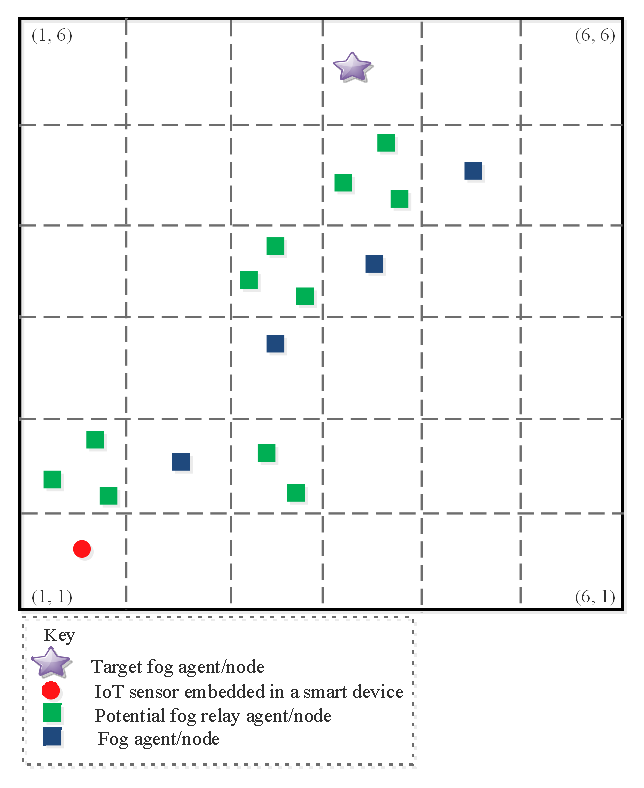
\includegraphics[width=3.5in]{fogmodel.eps}
 %where an .eps filename suffix will be assumed under latex,
% and a .pdf suffix will be assumed for pdflatex; or what has been declared
% via \DeclareGraphicsExtensions.
\caption{System model depicting the role of fog agents in a dynamic and heterogenous IoT environment.}
\label{fogmodel}
\end{figure}

\section{Application of Reinforcement Learning in CPS}

\subsection{Smart Grid}

\subsection{Intelligent Transport System}

\subsection{Smart Cities}


\section{Conclusion}\label{sec:conclusions}








% use section* for acknowledgment
%\section*{Acknowledgment}
%The authors would like to acknowledge the intellectual and material contributions of COMSATS Institute of Information Technology (CIIT) and The World Academy of Sciences (TWAS) in supporting the Fellowship (FR number: 3240293236).

% Can use something like this to put references on a page
% by themselves when using endfloat and the captionsoff option.
\ifCLASSOPTIONcaptionsoff
  \newpage
\fi

%\newpage

% trigger a \newpage just before the given reference
% number - used to balance the columns on the last page
% adjust value as needed - may need to be readjusted if
% the document is modified later
%\IEEEtriggeratref{8}
% The "triggered" command can be changed if desired:
%\IEEEtriggercmd{\enlargethispage{-5in}}

% references section

% can use a bibliography generated by BibTeX as a .bbl file
% BibTeX documentation can be easily obtained at:
% http://mirror.ctan.org/biblio/bibtex/contrib/doc/
% The IEEEtran BibTeX style support page is at:
% http://www.michaelshell.org/tex/ieeetran/bibtex/
%\bibliographystyle{IEEEtran}
% argument is your BibTeX string definitions and bibliography database(s)
%\bibliography{IEEEabrv,../bib/paper}
%
% <OR> manually copy in the resultant .bbl file
% set second argument of \begin to the number of references
% (used to reserve space for the reference number labels box)
\begin{thebibliography}{1}

\bibitem{Omoniwa2018}
B. Omoniwa, R. Hussain, M. A. Javed, S. H. Bouk and S. A. Malik, "Fog/Edge Computing-based IoT (FECIoT): Architecture, Applications, and Research Issues," in IEEE Internet of Things Journal.

\bibitem{Earley2015}
S. Earley, ``Analytics, Machine Learning, and the Internet of Things,'' \emph{IT Professional,} vol. 17, no. 1, pp. 10-13, Jan.-Feb. 2015.

\bibitem{Zhang18}
D. Zhang, X. Han and C. Deng,``Review on the research and practice of deep learning and reinforcement learning in smart grids,'' \emph{CSEE Journal of Power and Energy Systems,} vol. 4, no. 3, pp. 362-370, September 2018.

\bibitem{Watkins92}
C. J. C. H. Watkins and P. Dayan, Machine Learning (1992), Kluwer Academic Publishers, vol. 8: 279.

\bibitem{Wen15}
Z. Wen, D. O'Neill and H. Maei, ``Optimal Demand Response Using Device-Based Reinforcement Learning,'' \emph{IEEE Transactions on Smart Grid,} vol. 6, no. 5, pp. 2312-2324, Sept. 2015.

\bibitem{Sutton98}
R. S. Sutton, and A. G. Barto, \emph{Reinforcement learning - an introduction.} Cambridge, MA: MIT Press, 1998.

\bibitem{Zhu2018}
J. Zhu, Y. Song, D. Jiang and H. Song, ``A New Deep-Q-Learning-Based Transmission Scheduling Mechanism for the Cognitive Internet of Things,'' \emph{IEEE Internet of Things Journal,} vol. 5, no. 4, pp. 2375-2385, Aug. 2018.

\bibitem{Zhu2013}
J. Zhu, Z. Peng and F. Li, ``A transmission and scheduling scheme based on W-learning algorithm in wireless networks,'' \emph{2013 8th International Conference on Communications and Networking in China (CHINACOM),} Guilin, 2013, pp. 85-90.

\bibitem{Gai2018}
K. Gai, M. Qiu, ``Optimal resource allocation using reinforcement learning for IoT content-centric services,'' \emph{Applied Soft Computing,} vol. 70,
pp. 12-21, Sept. 2018.

\bibitem{Dusparic2009}
I. Dusparic and V. Cahill, ``Distributed W-Learning: Multi-Policy Optimization in Self-Organizing Systems,'' 2009 Third IEEE International Conference on Self-Adaptive and Self-Organizing Systems, San Francisco, CA, 2009, pp. 20-29.

\bibitem{Zhou2018}
L. Zhou, A. Swain and A. Ukil, ``Q-learning and Dynamic Fuzzy Q-learning Based Intelligent Controllers for Wind Energy Conversion Systems,'' \emph{2018 IEEE Innovative Smart Grid Technologies - Asia (ISGT Asia),} Singapore, 2018, pp. 103-108.

\bibitem{Park2016}
T. Park, N. Abuzainab and W. Saad, ``Learning How to Communicate in the Internet of Things: Finite Resources and Heterogeneity,'' \emph{IEEE Access,} vol. 4, pp. 7063-7073, 2016.

\bibitem{Hans2010}
A. Hans and S. Udluft, ``Ensembles of Neural Networks for Robust Reinforcement Learning,'' \emph{2010 Ninth International Conference on Machine Learning and Applications,} Washington, DC, 2010, pp. 401-406.

\bibitem{Nguyen2017}
D. D. Nguyen, H. X. Nguyen and L. B. White, ``Reinforcement Learning With Network-Assisted Feedback for Heterogeneous RAT Selection,'' \emph{IEEE Transactions on Wireless Communications,} vol. 16, no. 9, pp. 6062-6076, Sept. 2017.

\bibitem{Mohammadi2018}
M. Mohammadi, A. Al-Fuqaha, M. Guizani and J. Oh, ``Semisupervised Deep Reinforcement Learning in Support of IoT and Smart City Services,'' \emph{IEEE Internet of Things Journal,} vol. 5, no. 2, pp. 624-635, April 2018.

\bibitem{Alletto2016}
S. Alletto et al., ``An Indoor Location-Aware System for an IoT-Based Smart Museum,'' \emph{IEEE Internet of Things Journal,} vol. 3, no. 2, pp. 244-253, April 2016.
doi: 10.1109/JIOT.2015.2506258

\bibitem{Kolomvatsos2017}
K. Kolomvatsos, and C. Anagnostopoulos, ``Reinforcement Learning for Predictive Analytics in
Smart Cities,'' \emph{Informatics,} vol. 3, no. 16, June 2017.

\bibitem{Conti2017}
S. Conti, G. Faraci, R. Nicolosi, S. A. Rizzo and G. Schembra, ``Battery Management in a Green Fog-Computing Node: a Reinforcement-Learning Approach,'' \emph{IEEE Access,} vol. 5, pp. 21126-21138, 2017.

\bibitem{Mai2018}
L. Mai, N.-N. Dao, and M. Park, ``Real-time task assignment approach leveraging reinforcement learning with evolution strategies for long-term latency minimization in fog computing,'' \emph{Sensors,} vol. 18, no. 2830, Aug. 2018.

\bibitem{Kwok2004}
C. Kwok and D. Fox, ``Reinforcement learning for sensing strategies,'' \emph{2004 IEEE/RSJ International Conference on Intelligent Robots and Systems (IROS) (IEEE Cat. No.04CH37566),} Sendai, 2004, pp. 3158-3163 vol.4.

\bibitem{Li2015}
Y. Li, K. K. Chai, Y. Chen and J. Loo, ``Smart duty cycle control with reinforcement learning for machine to machine communications,'' \emph{2015 IEEE International Conference on Communication Workshop (ICCW),} London, 2015, pp. 1458-1463.

\bibitem{Li2014}
Y. Li, K. K. Chai, Y. Chen and J. Loo, ``Optimised delay-energy aware duty cycle control for IEEE 802.15.4 with cumulative acknowledgement,'' \emph{2014 IEEE 25th Annual International Symposium on Personal, Indoor, and Mobile Radio Communication (PIMRC),} Washington, DC, 2014, pp. 1051-1056.

\bibitem{Grammatopoulou2018}
M. Grammatopoulou, A. Kanellopoulos, and K. G. Vamvoudakis, ``A multi-step and resilient predictive Q-learning algorithm for IoT: a case study in water supply networks'', \emph{ACM Proceedings of the 8th International Conference on the Internet of Things,} Santa Barbara, California, 2018, pp. 1-8.

\bibitem{Debizet2018}
Y. Debizet, G. Lallement, F. Abouzeid, P. Roche and J. Autran, "Q-Learning-based Adaptive Power Management for IoT System-on-Chips with Embedded Power States," 2018 IEEE International Symposium on Circuits and Systems (ISCAS), Florence, 2018, pp. 1-5.

\bibitem{Khan2018}
M. I. Khan, M. M. Alam, Y. Le Moullec and E. Yaacoub, "Cooperative reinforcement learning for adaptive power allocation in device-to-device communication," 2018 IEEE 4th World Forum on Internet of Things (WF-IoT), Singapore, 2018, pp. 476-481.

\bibitem{routray2017}
S. K. Routray and Sharmila K. P., ``Routing in dynamically changing node location scenarios: A reinforcement learning approach,'' 2017 Third International Conference on Advances in Electrical, Electronics, Information, Communication and Bio-Informatics (AEEICB), Chennai, 2017, pp. 458-462.

\bibitem{Liu2017}
Y. Liu, L. Liu and W. Chen, "Intelligent traffic light control using distributed multi-agent Q learning," 2017 IEEE 20th International Conference on Intelligent Transportation Systems (ITSC), Yokohama, 2017, pp. 1-8.

\bibitem{Dias2016}
G. M. Dias, M. Nurchis and B. Bellalta, "Adapting sampling interval of sensor networks using on-line reinforcement learning," 2016 IEEE 3rd World Forum on Internet of Things (WF-IoT), Reston, VA, 2016, pp. 460-465.

\bibitem{Camelo2016}
M. Camelo and J. F. a. S. Latré, "A Scalable Parallel Q-Learning Algorithm for Resource Constrained Decentralized Computing Environments," 2016 2nd Workshop on Machine Learning in HPC Environments (MLHPC), Salt Lake City, UT, 2016, pp. 27-35.

\end{thebibliography}


% that's all folks
\end{document}


